\chapter{Technische aspecten}
\section{Machine Learning}
\subsection{Inleiding}
\npar Leren is een veelzijdig fenomeen dat bestaat uit  verschillende processen: het verkrijgen van declaratieve kennis, het ontwikkelen van motorische en cognitieve vaardigheden door instructie en ervaring, het organiseren van nieuwe kennis in algemene representaties en het ontdekken van nieuwe feiten via observatie en experimentatie.
\npar Sinds het begin van het computertijdperk proberen onderzoekers het menselijk leren na te bootsen en deze processen te vertalen naar de informatietheorie. Het machinaal leren is nog steeds een erg uitdagend doel in de kunstmatige intelligentie (KI).

\npar Deze vorm van KI is dus volledig data gedreven tegenover traditionele methoden die zich beroepen op handgemaakte regels. Het computerprogramma wordt niet expliciet geprogrammeerd om een taak uit te voeren maar vertrekt vanuit een algemeen model. Het model leert eerst uit voorbeelden en kan daarna voorspellingen maken op nieuwe invoer.

\npar We kunnen zeggen dat een computerprogramma of machine leert als het zijn performantie op een bepaalde taak verbetert met ervaring \cite{machine_overview}.  Het leren gebeurt door de optimalisatie van de parameters van het predictief model door middel van een algoritme uit de machine learning. Het model wordt een aantal voorbeelden gegeven om uit te leren: de trainset. De uitvoer van het model wordt ge\"evalueerd aan de hand van een prestatiemaat. Deze prestatiemaat vertelt hoe correct de voorspelling is en bepaalt de mate waarin het model verder gecorrigeerd dient te worden.

\npar Machine learning algoritmes kunnen opgedeeld worden in drie categori\"en op basis van leerstijl: gesuperviseerd, ongesuperviseerd en semi-gesuperviseerd leren. De supervisie slaat op het gebruik van de correcte uitgangswaarde tijdens het trainen.

\npar Een ongesuperviseerde leerstijl vertrekt uit een dataset zonder klasselabels of correcte voorspellingswaarde. Er wordt een model opgebouwd die bepaalde structuren deduceert. Dit kan zijn om algemene regels te extraheren, om redundantie te verminderen of om gegevens te groeperen volgens gelijkenis (clustering).

\npar Bij gesuperviseerde methodes wordt een trainset gebruikt die zowel de invoervector als de te voorspellen waarde bevat. Problemen die vaak via gesuperviseerd leren worden aangepakt zijn classificatie en regressie. Classificatie tracht ingevoerde voorbeelden in te delen in discrete categori\"en om bijvoorbeeld objecten te herkennen zoals in \cite{krizhevsky2012imagenet}. Bij regressie is de uitvoer van het model een continue variabele zoals bijvoorbeeld de prijs van een appartement gegeven zijn oppervlakte.

\npar Semi-gesuperviseerde methodes zijn een mengvorm van de voorgaande twee. De dataset is een mengeling van gelabelde en ongelabelde voorbeelden. Hierbij is er een gewenste indeling, weergegeven door de gelabelde data, maar het model moet zelf de indeling zien te maken.


\subsection{Gesuperviseerde classificatie}

\npar De machine learning in dit onderzoek valt onder de gesuperviseerde classificatie. Een classificatieprobleem kan algemeen als volgt worden omschreven:
\npar Gegeven een trainset T:
\begin{equation}
T = \{ ( x^{(n)}, y^{(n)})\},\quad x^{(n)}\in\mathbb{R}^D, y^{(n)}\in\{0,1,...,C\}, n=1,...,N
\end{equation}
met $x^{(n)}$ het n-de datavoorbeeld en $y^{(n)}$ zijn klasselabel. C staat voor het aantal discrete categori\"en of klasses, D het aantal dimensies van de invoervariabelen en N het aantal trainingsvoorbeelden. Nu kunnen we het classificatieprobleem uitdrukken als de benadering van een model $f$ met parameters $\theta$:
\begin{equation}\label{eq:classifier}
f(x,\theta) = y,\quad\forall(x,y) \in T
\end{equation}
zodat we na deze schatting vanuit $f$ en $\theta$ voorspellingen kunnen maken op basis van nieuwe data: $f(x_{nieuw},\theta)=y', \quad y' \in\{0,1,...C\}$

\npar Figuur \ref{alg-class-model} geeft een schematische weergave van de opbouw van een classificatiemodel. Het schatten van $f$ en $\theta$ wordt uitgevoerd door een techniek uit de machine learning en geeft ons het uiteindelijke predictief model $f(x,\theta) = y$. De samples worden meestal verwerkt voor ze als input worden doorgegeven aan het model. In het geval van classificatie van video en afbeeldingen worden er technieken uit de beeldverwerking gebruikt om relevante informatie uit het beeld te halen. Welke specifieke techniek er gebruikt wordt is een keuze die erg bewust moet gemaakt worden en een grote invloed heeft op de performantie van het classificatiemodel. Deze informatie wordt gebundeld in een featurevector ($x$) en aan het ML algoritme gegeven. Vanuit de verkregen featurevectoren en de kennis van het correcte klasselabel wordt het predictief model dan geoptimaliseerd.
\npar Eenmaal het model voldoende geleerd heeft kan het predictief model gebruikt worden in een productieomgeving om nieuwe voorbeelden, al dan niet correct, te classificeren.
\npar Het model dat in dit onderzoek gebruikt wordt is dat van het artificieel neuraal netwerk, een veel gebruikt predictief model voor classificatie. In sectie \ref{sec:ann} wordt deze techniek dan ook verder besproken.
\begin{figure}
	\centering
	\def\svgscale{0.85}
%	\def\svgwidth{\columnwidth}
	\input{figuren/figuur-classificatieML.pdf_tex}
	\singlespace \caption{Schematische weergave van het opstellen van een predictief model met behulp van machine learning technieken \label{alg-class-model}}
\end{figure}

\subsection{Overfitting}


\cite{dropout}

\section{Artificieel neuraal netwerk}\label{sec:ann}

\begin{figure}[ht]
	\begin{center}
		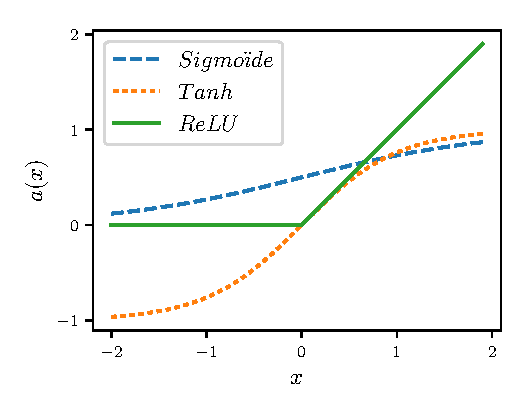
\includegraphics[width=8cm,keepaspectratio]{figuren/activatiefuncties.pdf}
		\singlespacing\caption{Weergave van de drie meest populaire activatiefuncties voor classificatie doeleinden \label{class-functies}}
	\end{center}
\end{figure}

\begin{figure}
	\centering
	\begin{subfigure}{.5\textwidth}
		\centering
		\input{figuren/neuron.pdf_tex}
		\caption{Artificieel neuron.}
		\label{neuron}
	\end{subfigure}%
	\begin{subfigure}{.5\textwidth}
		\centering
		\input{figuren/ANN-alg.pdf_tex}
		\caption{Artificieel neuraal netwerk}
		\label{fig:sub2}
	\end{subfigure}
	\caption{Een ANN met een invoerlaag, twee verborgen lagen en een softmax uitvoerlaag.}
	\label{fig:test}
\end{figure}

\subsection{Gradient descent}



\begin{equation}
\begin{aligned}
\textup{Sigmo\"ide unit:}\quad& a(x) = tanh(x)\\
\textup{Tanh unit:}\quad& a(x) = \frac{1}{x+exp(-x)}\\
\textup{Rectified Linear Unit (Relu):}\quad& a(x) = max(0,x)
\end{aligned}
\end{equation}

\npar Samenstelling van lineaire transformaties is zelf een lineaire transformatie
\section{Convolutioneel neuraal netwerk}
De vloek van de dimensionaliteit: 
\subsection{Tweedimensionale convolutie}
\subsection{Maximum pooling}
\section{Hyperparameters}
\subsection{Momentum}
\subsection{Dropout}